\subsection{Pozicijos nustatymas panaudojus telefoną}

Pirmas darbas apžvalgai yra \cite{willemsenconcept}, ``Concept for building a MEMS based indoor localization system''. Darbas pasiūlo galimos navigacinės sistemos prototipą, kuris remiasi inerciniais jutikliais. Kaip prototipo pagrindą buvo pasirinkit du mobilieji telefonai, kurie turi barometrą, pagreičio ir giroskopo jutiklį.

Darbas pradedamas prototipo pagrindo apžvalga, o konkrečiai nuo barometro. Barometras kaip matavimo įrenginys gali būti panaudotas pastato vidaus navigacijai, kurio pagalba galima nustatyti aukštą, kuriame yra stebimas objektas. Oro slėgis $p_i$ yra konvertuojamas į barometro aukščio formulę

\begin{equation}
    h_i = \Bigg( 1 - \sqrt[\leftroot{-2}\uproot{2}5.255]{ \frac{p_i}{1013.25} } \Bigg) \times \frac{288.15}{0.0065},
\end{equation}

Testavimo bazė buvo panaudotas \textit{HafenCity University} pastatas, kuris turėjo keturis aukštus. Duomenų surinkimo metu, jutiklis buvo perneštas per visus pastato aukštus su 4-3-2-1-1-2-3-4 seka. Rezultatai yra pateikiami \ref{fig:floor_detection_with_barometer_data} pavyzdyje.

\begin{figure}[H]
    \caption{Barometro naudojimas aukšto atpažinimui \cite{willemsenconcept}.}
    \label{fig:floor_detection_with_barometer_data}
    \centering
    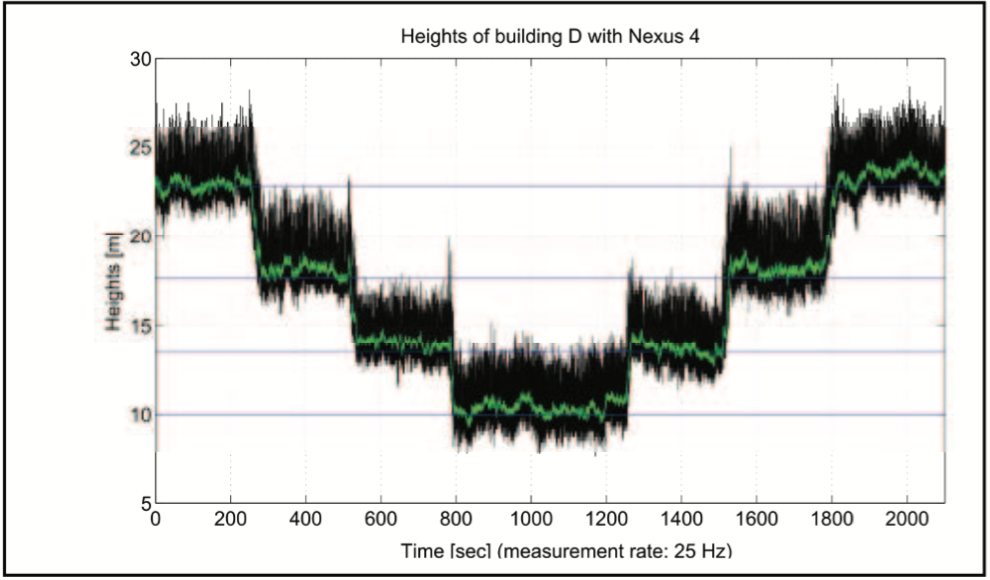
\includegraphics[width=300px]{img/floor_detection_with_barometer_data.png}
\end{figure}

Grafike pavaizduotos juodos linijos vaizduoja gryną signalą, žalia juosta žymi vidutinį signalo įvertį per $1~s$ laikotarpį. Rezultatai labai ryškiai parodo, kad barometras gali būti panaudotas aukštui nustatyti.

Toliau yra nagrinėjamas pagreičio jutiklio pritaikymo galimybės. Iškarto yra teigiama, jog dviguba integracija, kuri gali būti panaudota apskaičiuojant nukeliautą atstumą yra visiškai negalimas panaudoti matmuo, kadangi pagreičio jutiklis yra labai linkęs dreifuoti. To pasekoje, jutiklis yra panaudojamas tik kaip žingsnių matuoklis. Žingsniui nustatyti yra panaudojamas sekantis metodas. Pirmiausiai yra laukiama kuomet pagreičio pokyčio vertė įkopia į teigiamą pusę. Tuomet algoritmas laukia neigiamo gradiento signale. Kai tik jis yra randamas -- detektuojamas žingsnis. Taip pat yra panaudojamas verčių buferis (angl. \textit{buffer}), norint minimizuoti klaidingą žingsnio radimą.

Kaip ir bet kokį jutiklį, pagreičio jutiklį reikia kalibruoti, nors iš pirmo žvilgsnio žingsnių atpažinimui to nereikia, tačiau būtent akselerometro pozicija nusako ašių gradientą, todėl norint tiksliai žinoti ašių etaloną, reikalinga kalibravimas. Tam autoriai vietinės srities gravitacijos įverčių duomenų bazę. Kalibravimo metodas yra paremtas \cite{wendel2011integrierte} Kalman filtru.
